\documentclass[journal,12pt,twocolumn]{IEEEtran}
\usepackage{setspace}
\usepackage{gensymb}
\usepackage{caption}
%\usepackage{multirow}
%\usepackage{multicolumn}
%\usepackage{subcaption}
%\doublespacing
\singlespacing
\usepackage{csvsimple}
\usepackage{amsmath}
\usepackage{float}
\usepackage{multicol}
%\usepackage{enumerate}
\usepackage{amssymb}
%\usepackage{graphicx}
\usepackage{newfloat}
%\usepackage{syntax}
\usepackage{listings}
\usepackage{color}
\usepackage{tikz}
\usetikzlibrary{shapes,arrows}



%\usepackage{graphicx}
%\usepackage{amssymb}
%\usepackage{relsize}
%\usepackage[cmex10]{amsmath}
%\usepackage{mathtools}
%\usepackage{amsthm}
%\interdisplaylinepenalty=2500
%\savesymbol{iint}
%\usepackage{txfonts}
%\restoresymbol{TXF}{iint}
%\usepackage{wasysym}
\usepackage{amsthm}
\usepackage{mathrsfs}
\usepackage{txfonts}
\usepackage{stfloats}
\usepackage{cite}
\usepackage{cases}
\usepackage{mathtools}
\usepackage{caption}
\usepackage{enumerate}	
\usepackage{enumitem}
\usepackage{amsmath}
%\usepackage{xtab}
\usepackage{longtable}
\usepackage{multirow}
%\usepackage{algorithm}
%\usepackage{algpseudocode}
\usepackage{enumitem}
\usepackage{mathtools}
\usepackage{hyperref}
%\usepackage[framemethod=tikz]{mdframed}
\usepackage{listings}
    %\usepackage[latin1]{inputenc}                                 %%
    \usepackage{color}                                            %%
    \usepackage{array}                                            %%
    \usepackage{longtable}                                        %%
    \usepackage{calc}                                             %%
    \usepackage{multirow}                                         %%
    \usepackage{hhline}                                           %%
    \usepackage{ifthen}                                           %%
  %optionally (for landscape tables embedded in another document): %%
    \usepackage{lscape}     


\usepackage{url}
\def\UrlBreaks{\do\/\do-}


%\usepackage{stmaryrd}


%\usepackage{wasysym}
%\newcounter{MYtempeqncnt}
\DeclareMathOperator*{\Res}{Res}
%\renewcommand{\baselinestretch}{2}
\renewcommand\thesection{\arabic{section}}
\renewcommand\thesubsection{\thesection.\arabic{subsection}}
\renewcommand\thesubsubsection{\thesubsection.\arabic{subsubsection}}

\renewcommand\thesectiondis{\arabic{section}}
\renewcommand\thesubsectiondis{\thesectiondis.\arabic{subsection}}
\renewcommand\thesubsubsectiondis{\thesubsectiondis.\arabic{subsubsection}}

% correct bad hyphenation here
\hyphenation{op-tical net-works semi-conduc-tor}

%\lstset{
%language=C,
%frame=single, 
%breaklines=true
%}

%\lstset{
	%%basicstyle=\small\ttfamily\bfseries,
	%%numberstyle=\small\ttfamily,
	%language=Octave,
	%backgroundcolor=\color{white},
	%%frame=single,
	%%keywordstyle=\bfseries,
	%%breaklines=true,
	%%showstringspaces=false,
	%%xleftmargin=-10mm,
	%%aboveskip=-1mm,
	%%belowskip=0mm
%}

%\surroundwithmdframed[width=\columnwidth]{lstlisting}
\def\inputGnumericTable{}                                 %%
\lstset{
%language=C,
frame=single, 
breaklines=true,
columns=fullflexible
}
 

\begin{document}
%
\tikzstyle{block} = [rectangle, draw,
    text width=3em, text centered, minimum height=3em]
\tikzstyle{sum} = [draw, circle, node distance=3cm]
\tikzstyle{input} = [coordinate]
\tikzstyle{output} = [coordinate]
\tikzstyle{pinstyle} = [pin edge={to-,thin,black}]

\theoremstyle{definition}
\newtheorem{theorem}{Theorem}[section]
\newtheorem{problem}{Problem}
\newtheorem{proposition}{Proposition}[section]
\newtheorem{lemma}{Lemma}[section]
\newtheorem{corollary}[theorem]{Corollary}
\newtheorem{example}{Example}[section]
\newtheorem{definition}{Definition}[section]
%\newtheorem{algorithm}{Algorithm}[section]
%\newtheorem{cor}{Corollary}
\newcommand{\BEQA}{\begin{eqnarray}}
\newcommand{\EEQA}{\end{eqnarray}}
\newcommand{\define}{\stackrel{\triangle}{=}}
\bibliographystyle{IEEEtran}
%\bibliographystyle{ieeetr}
\providecommand{\nCr}[2]{\,^{#1}C_{#2}} % nCr
\providecommand{\nPr}[2]{\,^{#1}P_{#2}} % nPr
\providecommand{\mbf}{\mathbf}
\providecommand{\pr}[1]{\ensuremath{\Pr\left(#1\right)}}
\providecommand{\qfunc}[1]{\ensuremath{Q\left(#1\right)}}
\providecommand{\sbrak}[1]{\ensuremath{{}\left[#1\right]}}
\providecommand{\lsbrak}[1]{\ensuremath{{}\left[#1\right.}}
\providecommand{\rsbrak}[1]{\ensuremath{{}\left.#1\right]}}
\providecommand{\brak}[1]{\ensuremath{\left(#1\right)}}
\providecommand{\lbrak}[1]{\ensuremath{\left(#1\right.}}
\providecommand{\rbrak}[1]{\ensuremath{\left.#1\right)}}
\providecommand{\cbrak}[1]{\ensuremath{\left\{#1\right\}}}
\providecommand{\lcbrak}[1]{\ensuremath{\left\{#1\right.}}
\providecommand{\rcbrak}[1]{\ensuremath{\left.#1\right\}}}
\theoremstyle{remark}
\newtheorem{rem}{Remark}
\newcommand{\sgn}{\mathop{\mathrm{sgn}}}
%\providecommand{\abs}[1]{\left\vert#1\right\vert}
%\providecommand{\res}[1]{\Res\displaylimits_{#1}} 
%\providecommand{\norm}[1]{\left\Vert#1\right\Vert}
%\providecommand{\mtx}[1]{\mathbf{#1}}
%\providecommand{\mean}[1]{E\left[ #1 \right]}
\providecommand{\fourier}{\overset{\mathcal{F}}{ \rightleftharpoons}}
%\providecommand{\hilbert}{\overset{\mathcal{H}}{ \rightleftharpoons}}
\providecommand{\system}{\overset{\mathcal{H}}{ \longleftrightarrow}}
	%\newcommand{\solution}[2]{\textbf{Solution:}{#1}}
\newcommand{\solution}{\noindent \textbf{Solution: }}
\newcommand{\myvec}[1]{\ensuremath{\begin{pmatrix}#1\end{pmatrix}}}
\providecommand{\dec}[2]{\ensuremath{\overset{#1}{\underset{#2}{\gtrless}}}}
\DeclarePairedDelimiter{\ceil}{\lceil}{\rceil}
%\numberwithin{equation}{section}
%\numberwithin{problem}{subsection}
%\numberwithin{definition}{subsection}
\makeatletter
%\@addtoreset{figure}{section}
\makeatother
\let\StandardTheFigure\thefigure
%\renewcommand{\thefigure}{\theproblem.\arabic{figure}}
\renewcommand{\thefigure}{\thesection}
%\numberwithin{figure}{subsection}
%\numberwithin{equation}{subsection}
%\numberwithin{equation}{section}
%\numberwithin{equation}{problem}
%\numberwithin{problem}{subsection}
\numberwithin{problem}{section}
%%\numberwithin{definition}{subsection}
%\makeatletter
%\@addtoreset{figure}{problem}
%\makeatother
\makeatletter
\@addtoreset{table}{section}
\makeatother
\let\StandardTheFigure\thefigure
\let\StandardTheTable\thetable
\let\vec\mathbf
\numberwithin{equation}{section}
\vspace{3cm}
\title{%Convex Optimization in Python
	\logo{
	Random Numbers
	}
}
\author{Vedant Bhandare (CS21BTECH11007)}
%\title{
%	\logo{Matrix Analysis through Octave}{\begin{center}\includegraphics[scale=.24]{tlc}\end{center}}{}{HAMDSP}
%}
% paper title
% can use linebreaks \\ within to get better formatting as desired
%\title{Matrix Analysis through Octave}
%
%
% author names and IEEE memberships
% note positions of commas and nonbreaking spaces ( ~ ) LaTeX will not break
% a structure at a ~ so this keeps an author's name from being broken across
% two lines.
% use \thanks{} to gain access to the first footnote area
% a separate \thanks must be used for each paragraph as LaTeX2e's \thanks
% was not built to handle multiple paragraphs
%
% <-this % stops a space
%\thanks{J. Doe and J. Doe are with Anonymous University.}% <-this % stops a space
%\thanks{Manuscript received April 19, 2005; revised January 11, 2007.}}

% note the % following the last \IEEEmembership and also \thanks - 
% these prevent an unwanted space from occurring between the last author name
% and the end of the author line. i.e., if you had this:
% 
% \author{....lastname \thanks{...} \thanks{...} }
%                     ^------------^------------^----Do not want these spaces!
%
% a space would be appended to the last name and could cause every name on that
% line to be shifted left slightly. This is one of those "LaTeX things". For
% instance, "\textbf{A} \textbf{B}" will typeset as "A B" not "AB". To get
% "AB" then you have to do: "\textbf{A}\textbf{B}"
% \thanks is no different in this regard, so shield the last } of each \thanks
% that ends a line with a % and do not let a space in before the next \thanks.
% Spaces after \IEEEmembership other than the last one are OK (and needed) as
% you are supposed to have spaces between the names. For what it is worth,
% this is a minor point as most people would not even notice if the said evil
% space somehow managed to creep in.
% The paper headers
%\markboth{Journal of \LaTeX\ Class Files,~Vol.~6, No.~1, January~2007}%
%{Shell \MakeLowercase{\textit{et al.}}: Bare Demo of IEEEtran.cls for Journals}
% The only time the second header will appear is for the odd numbered pages
% after the title page when using the twoside option.
% 
% *** Note that you probably will NOT want to include the author's ***
% *** name in the headers of peer review papers.                   ***
% You can use \ifCLASSOPTIONpeerreview for conditional compilation here if
% you desire.
% If you want to put a publisher's ID mark on the page you can do it like
% this:
%\IEEEpubid{0000--0000/00\$00.00~\copyright~2007 IEEE}
% Remember, if you use this you must call \IEEEpubidadjcol in the second
% column for its text to clear the IEEEpubid mark.
% make the title area
\maketitle
%\tableofcontents
%\bigskip
\renewcommand{\thefigure}{\theenumi}
\renewcommand{\thetable}{\theenumi}
\begin{abstract}
This solution manual provides solutions and link to codes used for generation of random numbers.
\end{abstract}
%template ends here
\section{Uniform Random Variables}
\begin{enumerate}[label=\thesection.\arabic*
,ref=\thesection.\theenumi]
\item Generate $10^6$ samples of $U$ using a C program and save into a file called uni.dat .
\\
\solution\\ 
Download the following C code and run it to generate samples of U.
\begin{lstlisting}
wget https://github.com/TYCN129/AI1110-Assignments/blob/main/Manual%201/1.1/1.1.c
\end{lstlisting}
\item Load the uni.dat file into python and plot the empirical CDF of $U$ using the samples in uni.dat. The CDF is defined as
\begin{align}
F_{U}(x) = \pr{U \le x}
\end{align}
\\
\solution
Code used to plot empirical CDF of $U$
\begin{lstlisting}
wget https://github.com/TYCN129/AI1110-Assignments/blob/main/Manual%201/1.2/1.2.py
\end{lstlisting}
\begin{figure}[H]
    \includegraphics[width=\columnwidth]{update.png}
    \caption{CDF of $U$}
    \label{fig:my_label}
\end{figure}
\item Find a  theoretical expression for $F_{U}(x)$.\\
\solution\\
\begin{align}
    \displaystyle F_U(x) = \begin{cases} 
    0 & \text{$x < 0$} \\  
    x & \text{$0 \leq x \leq 1$} \\  
    1 & \text{$x > 1$}  
    \end{cases}
\end{align}

\begin{lstlisting}
wget https://github.com/TYCN129/AI1110-Assignments/blob/main/Manual%201/1.3/1.3.py
\end{lstlisting}
\item Find mean and variance of $U$.\\
\solution\\
Mean of Random Variable $U$ is given by,
\begin{equation}
E\sbrak{U} = \frac{1}{N}\sum_{i=1}^{N}U_i
\end{equation}
and its Variance is given by,
\begin{equation}
E\sbrak{\sbrak{U - E\sbrak{U}}^2} = E\sbrak{U^2} - \sbrak{E\sbrak{U}}^2
\end{equation}
Using the above two formulas, we get,\\
\begin{align}
\text{Mean of } U = 0.500031\\
\text{Variance of } U = 0.083247
\end{align}
Download and run the C code for mean and variance
\begin{lstlisting}
wget https://github.com/TYCN129/AI1110-Assignments/blob/main/Manual%201/1.4/1.4.c
\end{lstlisting}
\item Verify your result theoretically that
\begin{equation}
E\sbrak{U^k} = \int_{-\infty}^{\infty}x^kdF_{U}(x)
\end{equation}
\solution\\
For $k = 1$,
\begin{align}
E\sbrak{U} &= \int_{-\infty}^{\infty}xdF_{U}(x)\\
E\sbrak{U} &= \int_{0}^{1}xd(x)\\
E\sbrak{U} &= 0.5
\end{align}
Similarly, for $k = 2$,
\begin{align}
E\sbrak{U^2} &= 0.3333\\
\text{Variance} &= 0.0833
\end{align}
Thus the simulated and theoretical values of mean and variance of $U$ are approximately equal.
\end{enumerate}

\section{Central Limit Theorem}
\begin{enumerate}[label=\thesection.\arabic*
,ref=\thesection.\theenumi]
\item \solution\\
Download the following C code and run it to generate samples of $X$.
\begin{lstlisting}
wget https://github.com/TYCN129/AI1110-Assignments/blob/main/Manual%201/2.1/2.1.c
\end{lstlisting}
\item \solution

The plot was generated by running the following Python code
\begin{lstlisting}
wget https://github.com/TYCN129/AI1110-Assignments/blob/main/Manual%201/2.2./2.2.py
\end{lstlisting}
The CDF is a non-decreasing function with its range between 0 and 1. It will be continuous if PDF is finite.\\
\item {Load gau.dat in python and plot the empirical PDF of $X$ using the samples in gau.dat. The PDF of $X$ is defined as
\begin{align}
p_{X}\brak{x} = \frac{d}{dx}F_{X}\brak{x}
\label{eq:pdf_cdf}
\end{align}
What properties does the PDF have?}\\
\solution \\
The empirical PDF of $X$ is plotted by the Python code
\begin{lstlisting}
wget https://github.com/TYCN129/AI1110-Assignments/blob/main/Manual%201/2.3/2.3.py
\end{lstlisting}
The PDF takes non-negative values and area under its curve is 1.

\item Find the mean and variance of $X$ by writing a C program.
\\
\solution\\
Run the following C file
\begin{lstlisting}
wget https://github.com/TYCN129/AI1110-Assignments/blob/main/Manual%201/2.4/2.4.c
\end{lstlisting}
\begin{align}
E\sbrak{X}  &= 0.000630 \\
\text{var}\sbrak{X}  &= 1.000149
\end{align}

\item Given that 
\begin{align}
p_{X}\brak{x} = \frac{1}{\sqrt{2\pi}}\exp\brak{-\frac{x^2}{2}}, -\infty < x < \infty,
\end{align}
repeat the above exercise theoretically.\\
\solution\\
\begin{align}
    E\sbrak{X} &= \int_{-\infty}^{\infty}x p_{X}\brak{x} dx \\
    E\sbrak{X} &= \int_{-\infty}^{\infty}x
    \frac{1}{\sqrt{2\pi}}\exp\brak{-\frac{x^2}{2}} dx    
\end{align}
Taking $\frac{x^2}{2} = t$,
\begin{align}
    E\sbrak{X} &= -\int_{\infty}^{\infty}
    \frac{1}{\sqrt{2\pi}}\exp\brak{-t} dt\\
    E\sbrak{X} &= 0
\end{align}
To calculate variance,
\begin{align}
    var\sbrak{X} &= E\sbrak{(X - E\sbrak{X})^2}\\
    var\sbrak{X} &= E\sbrak{X^2}\\
    var\sbrak{X} &= \int_{-\infty}^{\infty}x^2 p_{X}\brak{x} dx \\
    var\sbrak{X} &= \int_{-\infty}^{\infty}x^2
    \frac{1}{\sqrt{2\pi}}\exp\brak{-\frac{x^2}{2}} dx 
\end{align}
We know that,
\begin{align}
    \int_{-\infty}^{\infty}x^2\exp\brak{-\frac{x^2}{2}} &= \sqrt{2\pi}\\
    var\sbrak{X} &= 1
\end{align}
\begin{figure}[h!]
    \centering
    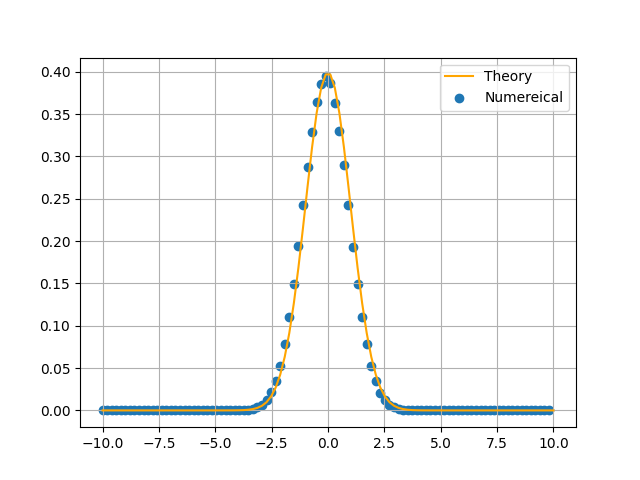
\includegraphics[width=\columnwidth]{Figure.png}
    \caption{PDF of $X$}
    \label{fig:my_label}
\end{figure}

\begin{figure}[h!]
    \centering
    \includegraphics[width=\columnwidth]{Figure_2.5_2.png}
    \caption{CDF of $X$}
    \label{fig:my_label}
\end{figure}

Theoretical expression for $X$,
\begin{align}
    F_X(x) &= 1 - Q(\frac{x - E\sbrak{X}}{var\sbrak{X}})\\
    F_X(x) &= 1 - Q(x)
\end{align}
The Python codes plot the CDF and PDF of $X$
\begin{lstlisting}
wget https://github.com/TYCN129/AI1110-Assignments/blob/main/Manual%201/2.5/2.5.py

wget https://github.com/TYCN129/AI1110-Assignments/blob/main/Manual%201/2.5/2.5_2.py
\end{lstlisting}
\end{enumerate}

\section{From Uniform to Other}
\begin{enumerate}[label=\thesection.\arabic*
,ref=\thesection.\theenumi]
    \item Generate samples of
\begin{align}
V = -2\ln\brak{1-U}
\end{align}
and plot its CDF. \\
\solution\\
Download and run the following code to generate samples of $V$
\begin{lstlisting}
wget https://github.com/TYCN129/AI1110-Assignments/blob/main/Manual%201/3.1/3.1.c
\end{lstlisting}
The following Python code plots CDF of $V$
\begin{lstlisting}
wget https://github.com/TYCN129/AI1110-Assignments/blob/main/Manual%201/3.1/3.1.py
\end{lstlisting}
\begin{figure}[h!]
    \centering
    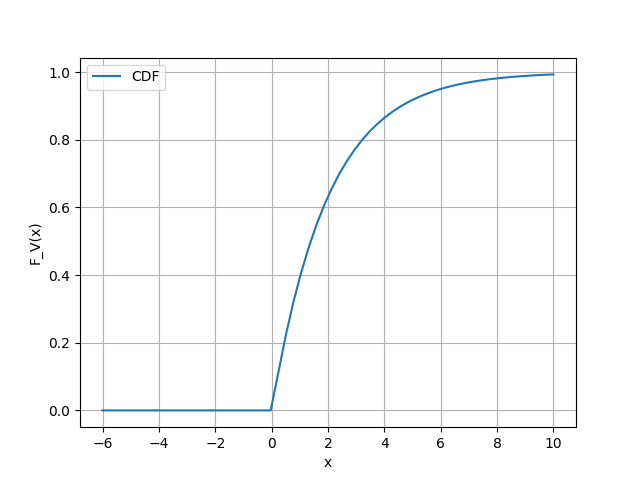
\includegraphics[width=\columnwidth]{Figure_3.1.png}
    \caption{The empirical CDF of $V$}
    \label{fig:my_label}
\end{figure}

\item Find a theoretical expression for $F_V\brak{x}$.
\\
\solution 
\begin{align}
	F_V\brak{x} &= Pr\brak{V\le x} \\
	F_V\brak{x} &= Pr\brak{-2\ln{\brak{1-U}} \le x}	\\
	F_V\brak{x} &= Pr\brak{\ln{\brak{1-U}} \ge -\frac{x}{2}}	\\
	F_V\brak{x} &= Pr\brak{1-U \ge \exp{\brak{-\frac{x}{2}} }}	\\
	F_V\brak{x} &= Pr\brak{U \le 1- \exp{\brak{-\frac{x}{2}} }} \\
	F_V\brak{x} &= F_U\brak{1- \exp{\brak{-\frac{x}{2}} }}		
\end{align}
\begin{small}
\begin{align}
	F_V\brak{x} &=
    \begin{cases}  
        0 & 1- \exp{\brak{-\frac{x}{2}} } < 0\\
        1- \exp{\brak{-\frac{x}{2}} } & 0 \le 1- \exp{\brak{-\frac{x}{2}} } \le 1 \\
        1 & 1 - \exp{\brak{-\frac{x}{2}} > 1 }
    \end{cases}
\end{align}
\end{small}
This simplifies to
\begin{align}
	F_V\brak{x} &=
    \begin{cases}  
        0 & x < 0\\
        1- \exp{\brak{-\frac{x}{2}}} & x \ge 0
    \end{cases}
    \label{eq:F_V}
\end{align}
The following python code plots the theoritical CDF
\begin{lstlisting}
wget https://github.com/TYCN129/AI1110-Assignments/blob/main/Manual%201/3.2/3.2.py
\end{lstlisting}
\begin{figure}[H]
    \centering
    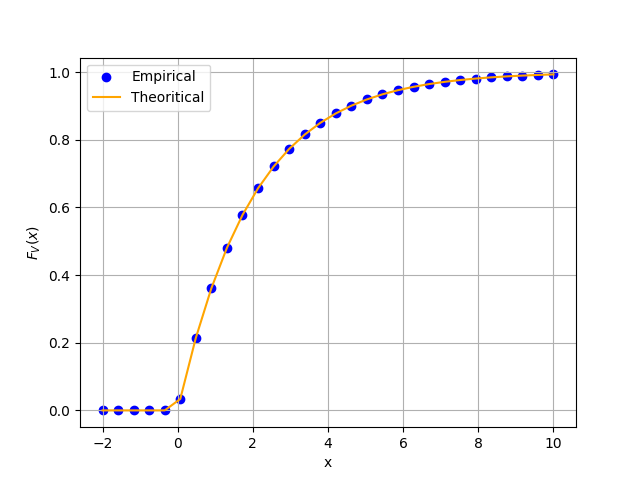
\includegraphics[width=\columnwidth]{Figure_3.2.png}
    \caption{CDF of $V$}
    \label{fig:my_label}
\end{figure}
\end{enumerate}

\section{Triangular Distribution}
\begin{enumerate}[label=\thesection.\arabic*
,ref=\thesection.\theenumi]
    \item Generate
    \begin{align}
        T = U_1 + U_2
    \end{align}

\solution\\
Download and run the following C code to generate tri.dat file.
\begin{lstlisting}
wget https://github.com/TYCN129/AI1110-Assignments/blob/main/Manual%201/4.1/4.1.c
\end{lstlisting}
\item Find the CDF of $T$.\\
\solution
\begin{figure}[h!]
    \centering
    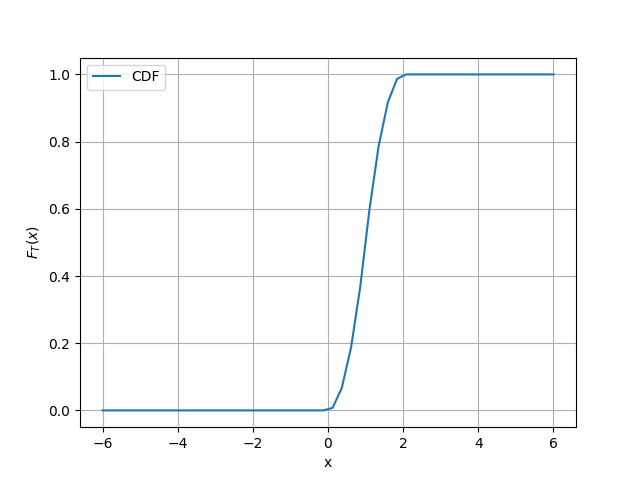
\includegraphics[width=\columnwidth]{Figure_4.2.png}
    \caption{CDF of $T$}
    \label{fig:my_label}
\end{figure}

The following code plots the CDF of $T$
\begin{lstlisting}
wget https://github.com/TYCN129/AI1110-Assignments/blob/main/Manual%201/4.2/4.2.py
\end{lstlisting}
\\
\item Find the CDF of $T$.\\
\solution
\begin{figure}[H]
    \centering
    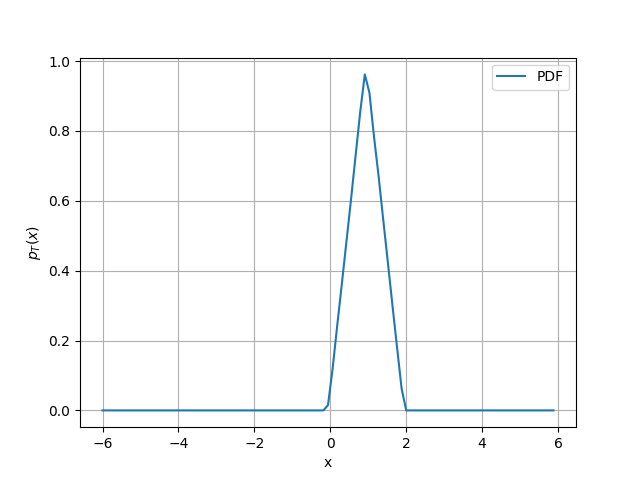
\includegraphics[width=\columnwidth]{Figure_4.3.png}
    \caption{PDF of $T$}
    \label{fig:my_label}
\end{figure}
The following code plots the PDF of $T$
\begin{lstlisting}
wget https://github.com/TYCN129/AI1110-Assignments/blob/main/Manual%201/4.3/4.3.py
\end{lstlisting}

\item Find the theoritical expressions for PDF and CDF of $T$.\\
\solution\\
\begin{align}
    p_T(x) &= p_{U_1 + U_2}(x) = p_{U_1}(x) * p_{U_2}(x)\\
    p_T(x) &= \int_{-\infty}^{\infty}p_{U_1}(\tau)p_{U_2}(x - \tau)d\tau\\
    p_T(x) &= \int_0^1p_{U_2}(x - \tau)d\tau
\end{align}
\begin{align}
    \displaystyle p_T(x) = \begin{cases} 
    0 & \text{$x \leq 0$} \\  
    \int_0^x 1d\tau & \text{$0 < x < 1$} \\  
    \int_{x - 1}^1 1d\tau & \text{$1 \leq x < 2$} \\
    0 & \text{$x > 2$}
    \end{cases}
\end{align}
\begin{align}
    \displaystyle p_T(x) = \begin{cases} 
    0 & \text{$x \leq 0$} \\  
    x & \text{$0 < x < 1$} \\  
    2 - x & \text{$1 \leq x < 2$} \\
    0 & \text{$x > 2$}
    \end{cases}
\end{align}
Expression for CDF can be obtained by integrating $p_T(x)$ w.r.t. $X$
\begin{align}
    \displaystyle F_T(x) = \begin{cases} 
    0 & \text{$x \leq 0$} \\  
    \frac{x^2}{2} & \text{$0 < x < 1$} \\  
    -\frac{x^2}{2} + 2x - 1 & \text{$1 \leq x < 2$} \\
    1 & \text{$x > 2$}
    \end{cases}
\end{align}

\item Verify the results through a plot.\\
\solution\\
\begin{figure}[h!]
    \centering
    \includegraphics[width=\columnwidth]{update1.png}
    \caption{Theoretical PDF of $T$}
    \label{fig:my_label}
\end{figure}
\begin{figure}[H]
    \centering
    \includegraphics[width=\columnwidth]{update2.png}
    \caption{The CDF of $T$}
    \label{fig:my_label}
\end{figure}
PDF and CDF plotted by the Python codes
\begin{lstlisting}
wget https://github.com/TYCN129/AI1110-Assignments/blob/main/Manual%201/4.5/4.5_1.py

wget https://github.com/TYCN129/AI1110-Assignments/blob/main/Manual%201/4.5/4.5_1.py
\end{lstlisting}
\end{enumerate}

\section{Maximul Likelihood}
\begin{enumerate}[label=\thesection.\arabic*
,ref=\thesection.\theenumi]
\item Generate equiprobable $X \in \cbrak{1,-1}$.\\
\solution\\
\\
Download and run the following codes to generate $X$.\\
\begin{lstlisting}
wget https://github.com/TYCN129/AI1110-Assignments/blob/main/Manual%201/5.1/5.1_X.c
\end{lstlisting}

\item Generate 
\begin{equation}
Y = AX+N,
\end{equation}
		where $A = 5$ dB,  and $N \sim \gauss{0}{1}$.\\
\solution\\
Download and run the following code to generate $Y$.
\begin{lstlisting}
wget https://github.com/TYCN129/AI1110-Assignments/tree/main/Manual%201/5.1/5.1_Y.c
\end{lstlisting}
\clearpage
\item Plot $Y$\\
\solution
\begin{figure}[H]
    \centering
    \includegraphics[width=\columnwidth]{Figure_5.2.png}
    \caption{Plot of $Y$}
    \label{fig:my_label}
\end{figure}
The Python code plots $Y$.
\begin{lstlisting}
wget https://github.com/TYCN129/AI1110-Assignments/blob/main/Manual%201/5.2/5.2.py
\end{lstlisting}
\item Guess how to estimate $X$ from $Y$\\
\solution\\
Estimate of $X = \hat{X}$ is found out from $Y$ by,
\begin{align}
    \hat{X} = \begin{cases}
    -1 & Y < 0\\
    1 & Y \geq 0
    \end{cases}
\end{align}

\item Find 
\begin{equation}
	P_{e|0} = \pr{\hat{X} = -1|X=1}
\end{equation}
and 
\begin{equation}
	P_{e|1} = \pr{\hat{X} = 1|X=-1}
\end{equation}
\solution\\
\begin{align}
	P_{e|0} &= \pr{\hat{X} = -1|X=1}\\
	&= 0.4998032
\end{align}
and 
\begin{align}
	P_{e|1} &= \pr{\hat{X} = 1|X=-1}\\
	&= 0.4995446
\end{align}

\item Find $P_e$ assuming $X$ has equiprobable symbols.\\
\solution\\
\begin{align}
    P_{e|0} &= Pr(\hat{X} = -1 | X = 1)\\
    &= Pr(AX + N < 0 | X = 1)\\
    &= Pr(N < -A)\\
    &= \int_{-\infty}^{-A}\frac{1}{\sqrt{2\pi}}\exp^{\frac{-x^2}{2}}\\
    &= \int_{A}^{\infty}\frac{1}{\sqrt{2\pi}}\exp^{\frac{-x^2}{2}}
    &= Q_N(A)
\end{align}
where, $Q_N(A)$ is the Q-function of Normal distribution. Similarly,
\begin{align}
    P_{e|1} = Q_N(A)
\end{align}
Thus,
\begin{align}
    P_e &= P_{e|0} \times Pr(X = 1) + P_{e|1} \times Pr(X = -1)\\
    P_e &= \frac{1}{2}\times P_{e|0} + \frac{1}{2}\times P_e{e|1}\\
    P_e &= \frac{P_{e|0} + P_{e|1}}{2}\\
    P_e &= Q_N(A)
\end{align}

\item Verify by plotting theoretical $P_e$ by varying $A$ from 0 to 10 dB\\
\solution\\
\begin{figure}[h!]
    \centering
    \includegraphics[width=\columnwidth]{Figure_5.7.png}
    \caption{Plot of $P_e$ with varying $A$}
    \label{fig:my_label}
\end{figure}
\begin{lstlisting}
wget https://github.com/TYCN129/AI1110-Assignments/tree/main/Manual%201/5.7
\end{lstlisting}

\item Now, consider a threshold $\delta$ while estimating $X$ from $Y$. Find the value of $\delta$ that maximizes the theoretical $P_e$.\\
\solution\\
Defining estimate of $X$ as,
\begin{align}
    \hat{X} &= \begin{cases}
    1 & Y > \delta\\
    -1 & Y < \delta
    \end{cases}\\
    P_{e|0} &= Pr(\hat{X} = -1 | X = 1)\\
    &= Pr(Y < \delta | X = 1)\\
    &= Pr(AX + N < \delta | X = 1)\\
    &= Pr(N < \delta - A)\\
    &= \int_{-\infty}^{\delta - A}\frac{1}{\sqrt{2\pi}}e^{\frac{-x^2}{2}}\\
    &= \int_{A - \delta}^{\infty}\frac{1}{\sqrt{2\pi}}e^{\frac{-x^2}{2}}\\
    &= Q_N(A - \delta)\\
    \intertext{Similarly,}\\
    P_{e|1} = Q_N(A + \delta)
\end{align}
Therefore,
\begin{align}
    P_e &= P(X = 1)\times P_{e|0} + P(X = -1)\times P_{e|1}\\
    &= \frac{Q_(A - \delta) + Q_N(A + \delta)}{2}
\end{align}
To maximize theoretical $P_e$, we differentiate equation (5.30) w.r.t $\delta$.\\
\begin{align}
    \frac{dP_e}{d\delta} &= \frac{1}{2} (\frac{1}{\sqrt{2\pi}} e^{-\frac{(\delta - A)^2}{2}} - \frac{1}{\sqrt{2\pi}} e^{-\frac{(A + \delta)^2}{2}})\\ 0 &= \frac{1}{2} (\frac{1}{\sqrt{2\pi}} e^{-\frac{(\delta - A)^2}{2}} - \frac{1}{\sqrt{2\pi}} e^{-\frac{(A + \delta)^2}{2}})\\
\intertext{Thus,}
    \delta &= 0
\end{align}

\item Repeat the above exercise when\\
\begin{equation}
    p_X(0) = p
\end{equation}
\solution\\
\begin{align}
    P_e &= P(X = 1)\times P_{e|0} + P(X = -1)\times P_{e|1}\\
    P_e &= pP_{e|0} + (1 - p)P_{e|1}
    \intertext{On differentiating both sides,}
    0 &= \frac{1}{2} (\frac{p}{\sqrt{2\pi}} e^{-\frac{(\delta - A)^2}{2}} - \frac{(1 - p)}{\sqrt{2\pi}} e^{-\frac{(A + \delta)^2}{2}})
    \intertext{Thus,}
    \delta &= \frac{1}{2A}ln\brak{\frac{(1 - p)}{p}}
\end{align}

\item Repeat the above exercise using the MAP criterion.\\
\solution\\
\begin{multline}
    p_Y(y) = p_{Y|X = 1}(y|1)\times P(X = 1) + \\
    p_{Y|X = -1}(y|-1)\times P(X = -1)\\
    = p_{N + A}(y)\times p + p_{N - A}(y)\times (1 - p)\\
\end{multline}
Here, $p_Y(y)$ is the PDF of $Y$, $p_{N + A}$ and $p_{N - A}$ are the PDF of shifted normal distribution.\\
\begin{align}
    p_Y(y) &= \frac{p}{\sqrt{2\pi}}e^{-\frac{(y + A)^2}{2}} + \frac{(1 - p)}{\sqrt{2\pi}}e^{-\frac{(y - A)^2}{2}}
\end{align}
Now, we need to find $p_{X|Y}(x|y)$ using the formula,
\begin{equation}
    p_{X|Y}(x|y) = \frac{p_{Y|X}(y|x) \times p_X(x)}{p_Y(y)}
\end{equation}
For $X = 1$,
\begin{align}
    p_{X|Y}(1|y) &= \frac{p_{Y|X}(y|1) \times p}{p_Y(y)}\\
    &= \frac{\frac{p}{\sqrt{2\pi}}e^{-\frac{(y + A)^2}{2}}}{\frac{p}{\sqrt{2\pi}}e^{-\frac{(y + A)^2}{2}} + \frac{(1 - p)}{\sqrt{2\pi}}e^{-\frac{(y - A)^2}{2}}}\\
    &= \frac{pe^{2Ay}}{pe^{2Ay} + (1 - p)}
    \intertext{Similarly, for $X = -1$,}
    p_{X|Y}(-1|y) &= \frac{p_{Y|X}(y|-1) \times (1 - p)}{p_Y(y)}\\
    &= \frac{\frac{(1 - p)}{\sqrt{2\pi}}e^{-\frac{(y - A)^2}{2}}}{\frac{p}{\sqrt{2\pi}}e^{-\frac{(y + A)^2}{2}} + \frac{(1 - p)}{\sqrt{2\pi}}e^{-\frac{(y - A)^2}{2}}}\\
    &= \frac{(1 - p)}{pe^{2Ay} + (1 - p)}
\end{align}
\begin{itemize}
    \item Case 1) $p_{X|Y}(1|y) > p_{X|Y}(-1|y)$
    \begin{align}
    \frac{pe^{2Ay}e^{2Ay}}{pe^{2Ay} + (1 - p)} &> \frac{(1 - p)}{pe^{2Ay} + (1 - p)}\\
    e^{-2Ay} &< \frac{p}{1 - p}\\
    y &> \frac{1}{2A}ln\brak{\frac{p}{1 - p}}
    \end{align}
Equation (5.50) holds good when $X = 1$.

\item Case 2) $p_{X|Y}(1|y) < p_{X|Y}(-1|y)$
    \begin{align}
    \frac{pe^{2Ay}}{pe^{2Ay} + (1 - p)} &< \frac{(1 - p)}{pe^{2Ay} + (1 - p)}\\
    e^{-2Ay} &> \frac{p}{1 - p}\\
    y &< \frac{1}{2A}ln\brak{\frac{p}{1 - p}}
    \end{align}
Equation (5.53) holds good when $X = -1$.
\end{itemize}

\end{enumerate}
\section{Gaussian to Other}
\begin{enumerate}[label=\thesection.\arabic*
,ref=\thesection.\theenumi]
\item
Let $X_1 \sim  \gauss{0}{1}$ and $X_2 \sim  \gauss{0}{1}$. Plot the CDF and PDF of

\begin{equation}
V = X_1^2 + X_2^2
\end{equation}

\solution\\
Download and run the C code to generate $V$.
\begin{lstlisting}
wget https://github.com/TYCN129/AI1110-Assignments/blob/main/Manual%201/6.1/6.1.c
\end{lstlisting}

\begin{figure}[h!]
    \centering
    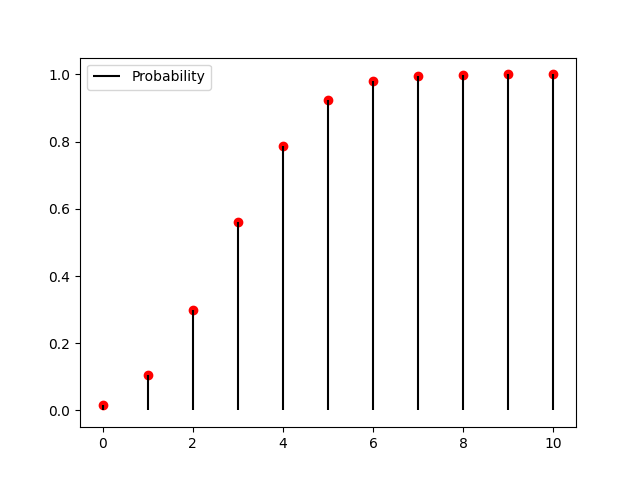
\includegraphics[width=\columnwidth]{CDF.png}
    \caption{CDF of $V$}
    \label{fig:my_label}
\end{figure}
\begin{figure}[H]
    \centering
    \includegraphics[width=\columnwidth]{PDF.png}
    \caption{PDF of $V$}
    \label{fig:my_label}
\end{figure}
\begin{lstlisting}
wget https://github.com/TYCN129/AI1110-Assignments/blob/main/Manual%201/6.1/CDF.py

wget https://github.com/TYCN129/AI1110-Assignments/blob/main/Manual%201/6.1/PDF.py
\end{lstlisting}
\item If
%
\begin{equation}
F_{V}(x) = 
\begin{cases}
1 - e^{-\alpha x} & x \geq 0 \\
0 & x < 0,
\end{cases}
\end{equation}
%
find $\alpha$.\\
\solution\\
Since $X_1$ and $X_2$ are i.i.d Normal Random Variables\\
Let $X_1=R\sin\theta$ and $X_2=R\cos\theta$\\
\begin{align}
              \intertext{Jacobian matrix is  given as follows}
              J                        & = \myvec{\frac{\delta x_1}{\delta r}                      & \frac{\delta x_1}{\delta \theta} \\ \frac{\delta x_2}{\delta r} & \frac{\delta x_2}{\delta \theta}}\\
              J                        & = \myvec{\cos\theta                                       & -R\sin\theta                     \\ \sin\theta & R\cos\theta}\\
              |J|                      & = R
              \intertext{Also, }
              \label{eq:frtheta}
              f_{r, \theta}(r, \theta) & = |J|f_{X_1, X_2}(x_1, x_2)                                                                  \\
              \intertext{Since, $X_1$ and $X_2$ are independent,}
              f_{X_1, X_2}(x_1, x_2)   & = f_{X_1}(x_1)f_{X_2}(x_2)                                                                   \\                                  \\
                                       & =\frac{1}{2\pi} e^{-\frac{(x_1^2+x_2^2)}{2}}                                                 \\
                                       & = \frac{1}{2\pi} e^{-\frac{r^2}{2}}
              \intertext{Put in \autoref{eq:frtheta}, we get,}
              f_{R, \theta}(r, \theta) & = \frac{r}{2\pi} e^{-\frac{r^2}{2}}
              \intertext{Now,}
              f_R(r)                   & = \int_0^{2\pi} f_{R, \theta}(r, \theta)                                                     \\
                                       & = \int_0^{2\pi} \frac{r}{2\pi} e^{-\frac{r^2}{2}} d\theta                                    \\
                                       & = r e^{-\frac{r^2}{2}}                                                                       \\
              \intertext{CDF is given by,}
              F_R(r) &= \int_0^r\exp{-\frac{r^2}{2}}\\
              &= 1 - \exp{\frac{-r^2}{2}}\\
              \intertext{And,}
              V                        & = X_1^2 + X_2^2                                                                              \\
                                       & = R^2
              \intertext{Now,}
              F_V(x)                   & = \pr{V\le x}                                                                                \\
                                       & = \pr{R^2 \le x}                                                                             \\
                                       & = \pr{R \le \sqrt{x}}                                                                        \\
              F_V(x)                   & = F_R(\sqrt{x})                                                                              \\
                                       & =\begin{cases}
                  0, & x < 0 \\
                  1 - e^{-\frac{x}{2}} & x \geq 0
              \end{cases}
          \end{align}

\begin{align}
    \alpha = \frac{1}{2}
\end{align}

\item Plot the CDF and PDF of $A$.
\begin{equation}
    A = \sqrt{V}
\end{equation}
\solution\\
Download the C code to generate $A = \sqrt{V}$\\
\begin{lstlisting}
wget https://github.com/TYCN129/AI1110-Assignments/blob/main/Manual%201/6.3/A.c
\end{lstlisting}

\begin{figure}[h!]
    \centering
    \includegraphics[width=\columnwidth]{6.3_CDF.png}
    \caption{CDF of $A$}
    \label{fig:my_label}
\end{figure}
\begin{figure}[H]
    \centering
    \includegraphics[width=\columnwidth]{6.3_PDF.png}
    \caption{PDF of $A$}
    \label{fig:my_label}
\end{figure}
\end{enumerate}
\end{document}
